For code

\begin{verbatim}
python $pwd/scan_info_efit.py #(0001)
\end{verbatim}




Image

As Figure \ref{fig:k_peak} shown, the peak of the growth rate is sensity of change of k near 0.

\begin{figure}[h] \centering
        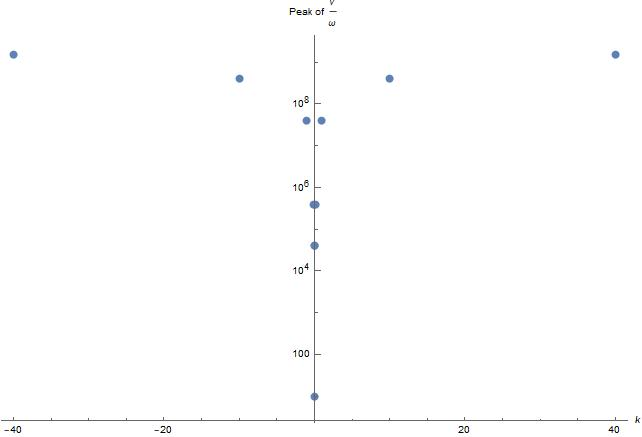
\includegraphics[width=1\textwidth]{Image/k_peak.jpg}
        \caption{The growth rate peak of MTM with changing k}
        \label{fig:k_peak}
\end{figure}


Chart

\begin{center}
            \begin{tabular}{ | m{5em} | m{2cm}| m{2cm} | m{2cm} |m{2cm} |m{2cm} | } 
                \hline
                Mode & $\frac{diff}{abs}$ & $\frac{Q_{EM}}{Q_{ES}}$ & $\frac{\chi_i}{\chi_e}$ & $\frac{D_e}{\chi_e}$ & $\frac{D_Z}{\chi_e}$\\
                \hline
                ITG & 1 & $<1$ & $\geq1$ & 1 & 1\\
                \hline
                ETG & 1 & $<1$ & 0 & 0 & 0\\
                \hline
                MTM & ~0.5 & $>1$ & 0 & 0 & 0\\
                \hline
                TEM & 1 & $<1$ & $\geq1$ & 1 & 1 \\
                \hline
                MHD & 0 & $<1$ & 1 & $\frac{2}{3}$ & $\frac{2}{3}$\\
                \hline
            \end{tabular}
            \label{ch:finger}
\end{center}



\begin{eqnarray}
\begin{aligned}
    k_{||}{}&=-i\nabla_{||}\\
    &=-i\textbf{b}\cdot \nabla \\
    &=-i\frac{B_z}{B_0}(\hat{e}_{\zeta}+\frac{r}{qR}\hat{e}_{\theta})\cdot(\hat{e}_{r}\frac{\partial}{\partial r}+\hat{e}_{\theta}\frac{1}{r}\frac{\partial}{\partial \theta}+\frac{1}{R}\hat{e}_{\zeta}\frac{\partial}{\partial \zeta})\\
    &=-i\frac{B_z}{B_0}(\frac{1}{qR}\frac{\partial}{\partial \theta }+\frac{1}{R}\frac{\partial}{\partial \zeta})\\
    &= -i \frac{B_z}{B_0}\frac{1}{qR}(\frac{\partial}{\partial \theta }+q\frac{\partial}{\partial \zeta})
\end{aligned}
\end{eqnarray}

\frac{\partial }{\partial z}